\documentclass[handout,nooutcomes,noauthor]{ximera}

\author{Bart Snapp}

%\usepackage{todonotes}
%\usepackage{mathtools} %% Required for wide table Curl and Greens
%\usepackage{cuted} %% Required for wide table Curl and Greens
\newcommand{\todo}{}

\usepackage{multicol}

\usepackage{esint} % for \oiint
\ifxake%%https://math.meta.stackexchange.com/questions/9973/how-do-you-render-a-closed-surface-double-integral
\renewcommand{\oiint}{{\large\bigcirc}\kern-1.56em\iint}
\fi

\graphicspath{
  {./}
  {ximeraTutorial/}
  {basicPhilosophy/}
  {functionsOfSeveralVariables/}
  {normalVectors/}
  {lagrangeMultipliers/}
  {vectorFields/}
  {greensTheorem/}
  {shapeOfThingsToCome/}
  {dotProducts/}
  {partialDerivativesAndTheGradientVector/}
  {../ximeraTutorial/}
  {../productAndQuotientRules/exercises/}
  {../motionAndPathsInSpace/exercises/}
  {../normalVectors/exercisesParametricPlots/}
  {../continuityOfFunctionsOfSeveralVariables/exercises/}
  {../partialDerivativesAndTheGradientVector/exercises/}
  {../directionalDerivativeAndChainRule/exercises/}
  {../commonCoordinates/exercisesCylindricalCoordinates/}
  {../commonCoordinates/exercisesSphericalCoordinates/}
  {../greensTheorem/exercisesCurlAndLineIntegrals/}
  {../greensTheorem/exercisesDivergenceAndLineIntegrals/}
  {../shapeOfThingsToCome/exercisesDivergenceTheorem/}
  {../greensTheorem/}
  {../shapeOfThingsToCome/}
  {../separableDifferentialEquations/exercises/}
  {../dotproducts/}
  {../functionsOfSeveralVariables/}
  {../lagrangeMultipliers/}
  {../partialDerivativesAndTheGradientVector/}
  {../normalVectors/}
  {../vectorFields/}
}
\def\xmNotExpandableAsAccordion{true}

\newcommand{\mooculus}{\textsf{\textbf{MOOC}\textnormal{\textsf{ULUS}}}}

\usepackage{tkz-euclide}\usepackage{tikz}
\usepackage{tikz-cd}
\usetikzlibrary{arrows}
\tikzset{>=stealth,commutative diagrams/.cd,
  arrow style=tikz,diagrams={>=stealth}} %% cool arrow head
\tikzset{shorten <>/.style={ shorten >=#1, shorten <=#1 } } %% allows shorter vectors

\usetikzlibrary{backgrounds} %% for boxes around graphs
\usetikzlibrary{shapes,positioning}  %% Clouds and stars
\usetikzlibrary{matrix} %% for matrix
\usepgfplotslibrary{polar} %% for polar plots
\usepgfplotslibrary{fillbetween} %% to shade area between curves in TikZ
%\usetkzobj{all} %% obsolete

\usepackage[makeroom]{cancel} %% for strike outs
%\usepackage{mathtools} %% for pretty underbrace % Breaks Ximera
%\usepackage{multicol}
\usepackage{pgffor} %% required for integral for loops

\usepackage{tkz-tab}  %% for sign charts

%% http://tex.stackexchange.com/questions/66490/drawing-a-tikz-arc-specifying-the-center
%% Draws beach ball
\tikzset{pics/carc/.style args={#1:#2:#3}{code={\draw[pic actions] (#1:#3) arc(#1:#2:#3);}}}



\usepackage{array}
\setlength{\extrarowheight}{+.1cm}
\newdimen\digitwidth
\settowidth\digitwidth{9}
\def\divrule#1#2{
\noalign{\moveright#1\digitwidth
\vbox{\hrule width#2\digitwidth}}}





\newcommand{\RR}{\mathbb R}
\newcommand{\R}{\mathbb R}
\newcommand{\N}{\mathbb N}
\newcommand{\Z}{\mathbb Z}

\newcommand{\sagemath}{\textsf{SageMath}}


\renewcommand{\d}{\,d}
%\def\d{\mathop{}\!d}
%\def\d{\,d}

\AddToHook{begindocument}{%
  \renewcommand{\d}{\,d}     % lualatex redefines \d to underdot !!!
}

\pgfplotsset{
    every axis/.style={
        scale only axis,
        enlargelimits=false,
        trim axis left,
        trim axis right,
        clip=true,
    }
}

\newcommand{\dd}[2][]{\frac{\d #1}{\d #2}}
\newcommand{\pp}[2][]{\frac{\partial #1}{\partial #2}}
\renewcommand{\l}{\ell}
\newcommand{\ddx}{\frac{d}{\d x}}

\newcommand{\zeroOverZero}{\ensuremath{\boldsymbol{\tfrac{0}{0}}}}
\newcommand{\inftyOverInfty}{\ensuremath{\boldsymbol{\tfrac{\infty}{\infty}}}}
\newcommand{\zeroOverInfty}{\ensuremath{\boldsymbol{\tfrac{0}{\infty}}}}
\newcommand{\zeroTimesInfty}{\ensuremath{\small\boldsymbol{0\cdot \infty}}}
\newcommand{\inftyMinusInfty}{\ensuremath{\small\boldsymbol{\infty - \infty}}}
\newcommand{\oneToInfty}{\ensuremath{\boldsymbol{1^\infty}}}
\newcommand{\zeroToZero}{\ensuremath{\boldsymbol{0^0}}}
\newcommand{\inftyToZero}{\ensuremath{\boldsymbol{\infty^0}}}



\newcommand{\numOverZero}{\ensuremath{\boldsymbol{\tfrac{\#}{0}}}}
\newcommand{\dfn}{\textbf}
%\newcommand{\unit}{\,\mathrm}
\newcommand{\unit}{\mathop{}\!\mathrm}
\newcommand{\eval}[1]{\bigg[ #1 \bigg]}
\newcommand{\seq}[1]{\left( #1 \right)}
\renewcommand{\epsilon}{\varepsilon}
\renewcommand{\phi}{\varphi}


\renewcommand{\iff}{\Leftrightarrow}

\DeclareMathOperator{\arccot}{arccot}
\DeclareMathOperator{\arcsec}{arcsec}
\DeclareMathOperator{\arccsc}{arccsc}
\DeclareMathOperator{\si}{Si}
\DeclareMathOperator{\scal}{scal}
\DeclareMathOperator{\sign}{sign}


%% \newcommand{\tightoverset}[2]{% for arrow vec
%%   \mathop{#2}\limits^{\vbox to -.5ex{\kern-0.75ex\hbox{$#1$}\vss}}}
\newcommand{\arrowvec}[1]{{\overset{\rightharpoonup}{#1}}}
%\renewcommand{\vec}[1]{\arrowvec{\mathbf{#1}}}
\renewcommand{\vec}[1]{{\overset{\boldsymbol{\rightharpoonup}}{\mathbf{#1}}}\hspace{0in}}

\newcommand{\point}[1]{\left(#1\right)} %this allows \vector{ to be changed to \vector{ with a quick find and replace
\newcommand{\pt}[1]{\mathbf{#1}} %this allows \vec{ to be changed to \vec{ with a quick find and replace
\newcommand{\Lim}[2]{\lim_{\point{#1} \to \point{#2}}} %Bart, I changed this to point since I want to use it.  It runs through both of the exercise and exerciseE files in limits section, which is why it was in each document to start with.

\DeclareMathOperator{\proj}{\mathbf{proj}}
\newcommand{\veci}{{\boldsymbol{\hat{\imath}}}}
\newcommand{\vecj}{{\boldsymbol{\hat{\jmath}}}}
\newcommand{\veck}{{\boldsymbol{\hat{k}}}}
\newcommand{\vecl}{\vec{\boldsymbol{\l}}}
\newcommand{\uvec}[1]{\mathbf{\hat{#1}}}
\newcommand{\utan}{\mathbf{\hat{t}}}
\newcommand{\unormal}{\mathbf{\hat{n}}}
\newcommand{\ubinormal}{\mathbf{\hat{b}}}

\newcommand{\dotp}{\bullet}
\newcommand{\cross}{\boldsymbol\times}
\newcommand{\grad}{\boldsymbol\nabla}
\newcommand{\divergence}{\grad\dotp}
\newcommand{\curl}{\grad\cross}
%\DeclareMathOperator{\divergence}{divergence}
%\DeclareMathOperator{\curl}[1]{\grad\cross #1}
\newcommand{\lto}{\mathop{\longrightarrow\,}\limits}

\renewcommand{\bar}{\overline}

\colorlet{textColor}{black}
\colorlet{background}{white}
\colorlet{penColor}{blue!50!black} % Color of a curve in a plot
\colorlet{penColor2}{red!50!black}% Color of a curve in a plot
\colorlet{penColor3}{red!50!blue} % Color of a curve in a plot
\colorlet{penColor4}{green!50!black} % Color of a curve in a plot
\colorlet{penColor5}{orange!80!black} % Color of a curve in a plot
\colorlet{penColor6}{yellow!70!black} % Color of a curve in a plot
\colorlet{fill1}{penColor!20} % Color of fill in a plot
\colorlet{fill2}{penColor2!20} % Color of fill in a plot
\colorlet{fillp}{fill1} % Color of positive area
\colorlet{filln}{penColor2!20} % Color of negative area
\colorlet{fill3}{penColor3!20} % Fill
\colorlet{fill4}{penColor4!20} % Fill
\colorlet{fill5}{penColor5!20} % Fill
\colorlet{gridColor}{gray!50} % Color of grid in a plot

\newcommand{\surfaceColor}{violet}
\newcommand{\surfaceColorTwo}{redyellow}
\newcommand{\sliceColor}{greenyellow}




\pgfmathdeclarefunction{gauss}{2}{% gives gaussian
  \pgfmathparse{1/(#2*sqrt(2*pi))*exp(-((x-#1)^2)/(2*#2^2))}%
}


%%%%%%%%%%%%%
%% Vectors
%%%%%%%%%%%%%

%% Simple horiz vectors
\renewcommand{\vector}[1]{\left\langle #1\right\rangle}


%% %% Complex Horiz Vectors with angle brackets
%% \makeatletter
%% \renewcommand{\vector}[2][ , ]{\left\langle%
%%   \def\nextitem{\def\nextitem{#1}}%
%%   \@for \el:=#2\do{\nextitem\el}\right\rangle%
%% }
%% \makeatother

%% %% Vertical Vectors
%% \def\vector#1{\begin{bmatrix}\vecListA#1,,\end{bmatrix}}
%% \def\vecListA#1,{\if,#1,\else #1\cr \expandafter \vecListA \fi}

%%%%%%%%%%%%%
%% End of vectors
%%%%%%%%%%%%%

%\newcommand{\fullwidth}{}
%\newcommand{\normalwidth}{}



%% makes a snazzy t-chart for evaluating functions
%\newenvironment{tchart}{\rowcolors{2}{}{background!90!textColor}\array}{\endarray}

%%This is to help with formatting on future title pages.
\newenvironment{sectionOutcomes}{}{}



%% Flowchart stuff
%\tikzstyle{startstop} = [rectangle, rounded corners, minimum width=3cm, minimum height=1cm,text centered, draw=black]
%\tikzstyle{question} = [rectangle, minimum width=3cm, minimum height=1cm, text centered, draw=black]
%\tikzstyle{decision} = [trapezium, trapezium left angle=70, trapezium right angle=110, minimum width=3cm, minimum height=1cm, text centered, draw=black]
%\tikzstyle{question} = [rectangle, rounded corners, minimum width=3cm, minimum height=1cm,text centered, draw=black]
%\tikzstyle{process} = [rectangle, minimum width=3cm, minimum height=1cm, text centered, draw=black]
%\tikzstyle{decision} = [trapezium, trapezium left angle=70, trapezium right angle=110, minimum width=3cm, minimum height=1cm, text centered, draw=black]


\title[Collaborate:]{Describing regions}

\begin{document}
\begin{abstract}
  We describe areas and volumes of regions using iterated integrals.
\end{abstract}
\maketitle

\textbf{Work in groups of 3--4, writing your answers on a separate
  sheet of paper.}

\section{Trivial regions}


\begin{problem}
  Without doing \textbf{any} integrals, evaluate
  \[
  \iint_R \d A
  \]
  where
  \[
  R =\{(x,y):-2\le x\le 4 \text{ and } -6\le y\le 1\}.
  \]
\end{problem}


\begin{problem}
  Without doing \textbf{any} integrals, evaluate
  \[
  \iiint_R \d V
  \]
  where
  \[
  R =\{(x,y,z):-4\le x\le 3, 
    -1\le y\le 5,\text{ and, } -3\le z\le 2\}.
  \]
\end{problem}

\section{Two-dimensional regions}

\begin{problem}
  Consider the region
  \[
  R=\{(x,y):0\le x\le 2+\cos(y)\text{ and }0<y<2\pi\}
  \]
  \begin{image}[1.75in]
    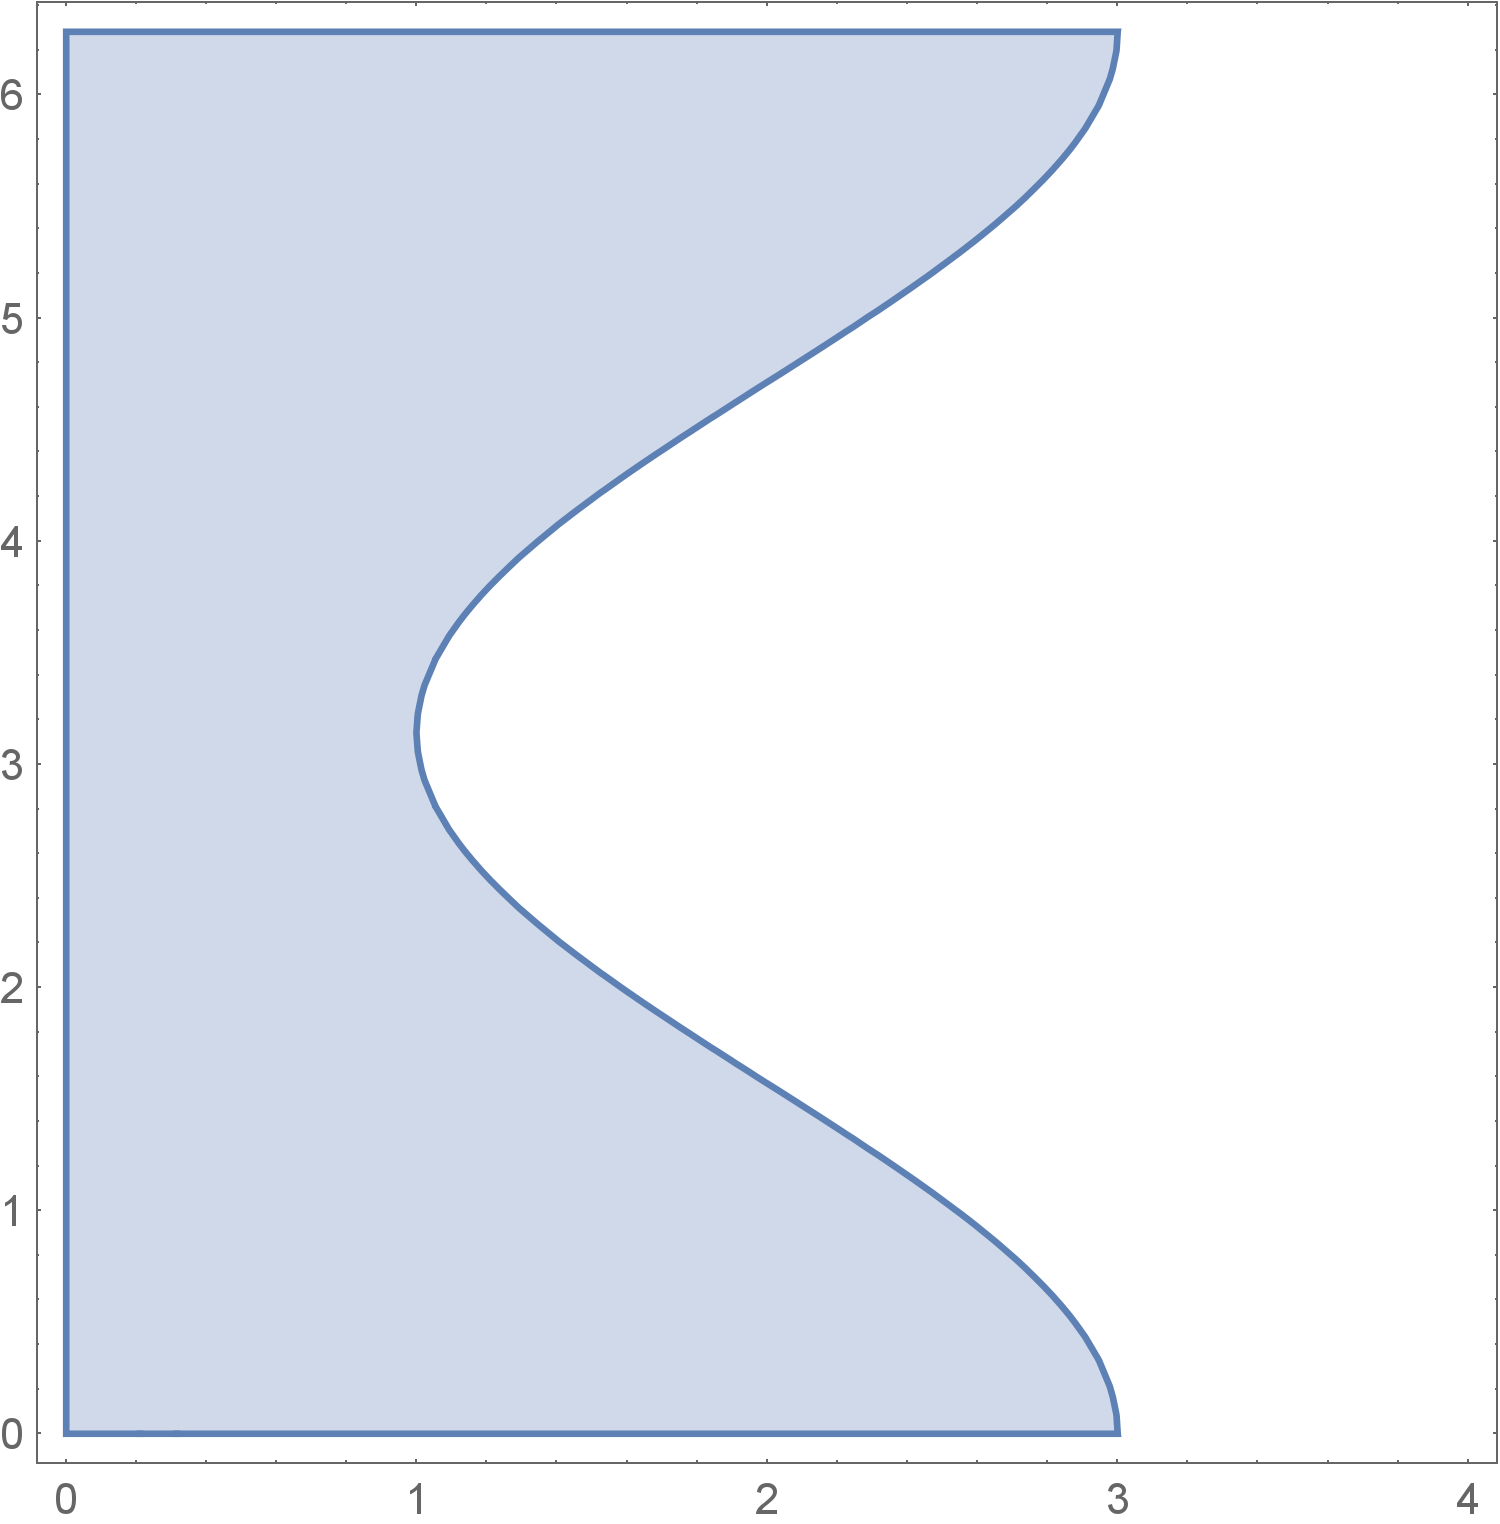
\includegraphics{region.png}
  \end{image}
  Compute the area of this region with an iterated integral where one
  integrates first with respect to $x$ and next integrates with
  respect to $y$.
  
  \textbf{As a challenge}, compute the area with an iterated integral
  where one integrates first with respect to $y$ and next integrates
  with respect to $x$.
\end{problem}


\begin{problem}
  Consider the region
   \begin{image}[2.5in]
    \begin{tikzpicture}
      \begin{axis}[
          tick label style={font=\scriptsize},
          axis y line=middle,axis x line=middle,
          name=myplot,
	  xtick={-1.5,-1,...,1.5},
	  ytick={-1.5,-1,...,1.5},
          grid = major,
          ymin=-1.5,ymax=1.5,%
	  xmin=-1.5,xmax=1.5,
          rounded corners=.5pt
        ]
        \draw [ultra thick,fill=fill1,draw=penColor] (axis cs: 0,-1) -- (axis cs: 1,1)-- (axis cs: -1,1)  -- cycle;
        
      \end{axis}
      
      \node [right] at (myplot.right of origin) {\scriptsize $x$};
      \node [above] at (myplot.above origin) {\scriptsize $y$};
    \end{tikzpicture}
   \end{image}
   \begin{enumerate}
   \item Compute the area of this region with an iterated integral
     where one integrates first with respect to $y$ and next
     integrates with respect to $x$.
   \item Compute the area of this region with an iterated integral
     where one integrates first with respect to $x$ and next
     integrates with respect to $y$.
   \end{enumerate}
\end{problem}

\begin{problem}
  Consider the ellipse centered at the origin:
  \begin{image}[2in]
    \begin{tikzpicture}
      \begin{axis}[
          tick label style={font=\scriptsize},
          axis y line=middle,axis x line=middle,
          name=myplot,axis on top,
	  xtick={-4,-3,...,4},
	  ytick={-1.5,-1,...,1.5},
          %grid = major,
          ymin=-1.5,ymax=1.5,%
	  xmin=-4.5,xmax=4.5,
          rounded corners=.5pt
        ]
        \addplot[penColor, fill= fill1,ultra thick,domain=0:360,samples=200] ({4*cos(x)},{1*sin(x)});
        
        
      \end{axis}
      
      \node [right] at (myplot.right of origin) {\scriptsize $x$};
      \node [above] at (myplot.above origin) {\scriptsize $y$};
    \end{tikzpicture}
  \end{image}
  Recall that the implicit formula for an ellipse is given by
  \[
  \left(\frac{x-x_0}{a}\right)^2 + \left(\frac{y-y_0}{b}\right)^2 = 1.
  \]
  \begin{enumerate}
   \item Compute the area of this region with an iterated integral
     where one integrates first with respect to $y$ and next
     integrates with respect to $x$.
   \item Compute the area of this region with an iterated integral
     where one integrates first with respect to $x$ and next
     integrates with respect to $y$.
   \end{enumerate}
\end{problem}

\begin{problem}
  Consider the following region:
  \begin{image}[2in]
    \begin{tikzpicture}
      \begin{axis}[
          tick label style={font=\scriptsize},
          axis y line=middle,axis x line=middle,
          name=myplot,axis on top,
	  xtick={-1.5,-1,...,1.5},
	  ytick={-.5,0,...,1.5},
          %grid = major,
          ymin=-.5,ymax=1.5,%
	  xmin=-1.5,xmax=1.5,
          rounded corners=.5pt
        ]
        \addplot[draw=none, fill= fill1,domain=-1:1] {1}\closedcycle;
        \addplot[penColor, fill= fill1,ultra thick,domain=45:135] ({(sqrt(2)) * cos(x)},{(sqrt(2))*sin(x)});
        \addplot[draw=none, fill= white,ultra thick,domain=0:1] {x}\closedcycle;
        \addplot[draw=none, fill=white,ultra thick,domain=-1:0] {-x}\closedcycle;

        \addplot[mark=*,penColor] coordinates {(1,1)};

        \addplot[penColor,ultra thick,domain=0:1] {x};
        \addplot[penColor,ultra thick,domain=-1:0] {-x};

        \node [right] at (axis cs: 1,1) {$(1,1)$};
        
      \end{axis}
      
      \node [right] at (myplot.right of origin) {\scriptsize $x$};
      \node [above] at (myplot.above origin) {\scriptsize $y$};
    \end{tikzpicture}
  \end{image}
  The largest $y$-value of the region is $y=\sqrt{2}$. 
  \begin{enumerate}
  \item Compute the area of this region with an iterated integral
    where one integrates first with respect to $y$ and next integrates
    with respect to $x$.
  \item Compute the area of this region with an iterated integral
    where one integrates first with respect to $x$ and next integrates
    with respect to $y$.
  \end{enumerate}
\end{problem}




\section{Three-dimensional regions}


\begin{problem}
  Consider the region bounded by the planes:
  \begin{itemize}
  \item $x=0$
  \item $y=0$
  \item $z=0$
  \item $6x+3y+2z = 24$
  \end{itemize}
  Sketch this region and set-up \textbf{six} iterated integrals that
  compute the volume of this solid, all which integrate in a different
  order.
\end{problem}


\begin{problem}
  Consider the region:
  \[
  R=\{(x,y,z): 0 \le x \le 1, -1\le y \le 0, 0\le z\le y^2\}
  \]
  \begin{image}[2in]
    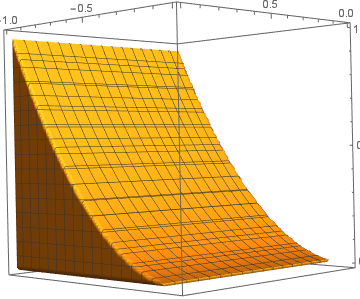
\includegraphics{threeRegion2.png}
  \end{image}
  Set up \textbf{six} iterated integrals that compute the volume of this solid,
  all which integrate in a different order.
\end{problem}

\begin{problem}
  Consider the region:
  \[
  R=\{(x,y,z): 0 \le x \le 1, \sqrt{x}\le y \le 1, 0\le z\le 1-y\}
  \]
  \begin{image}[2in]
    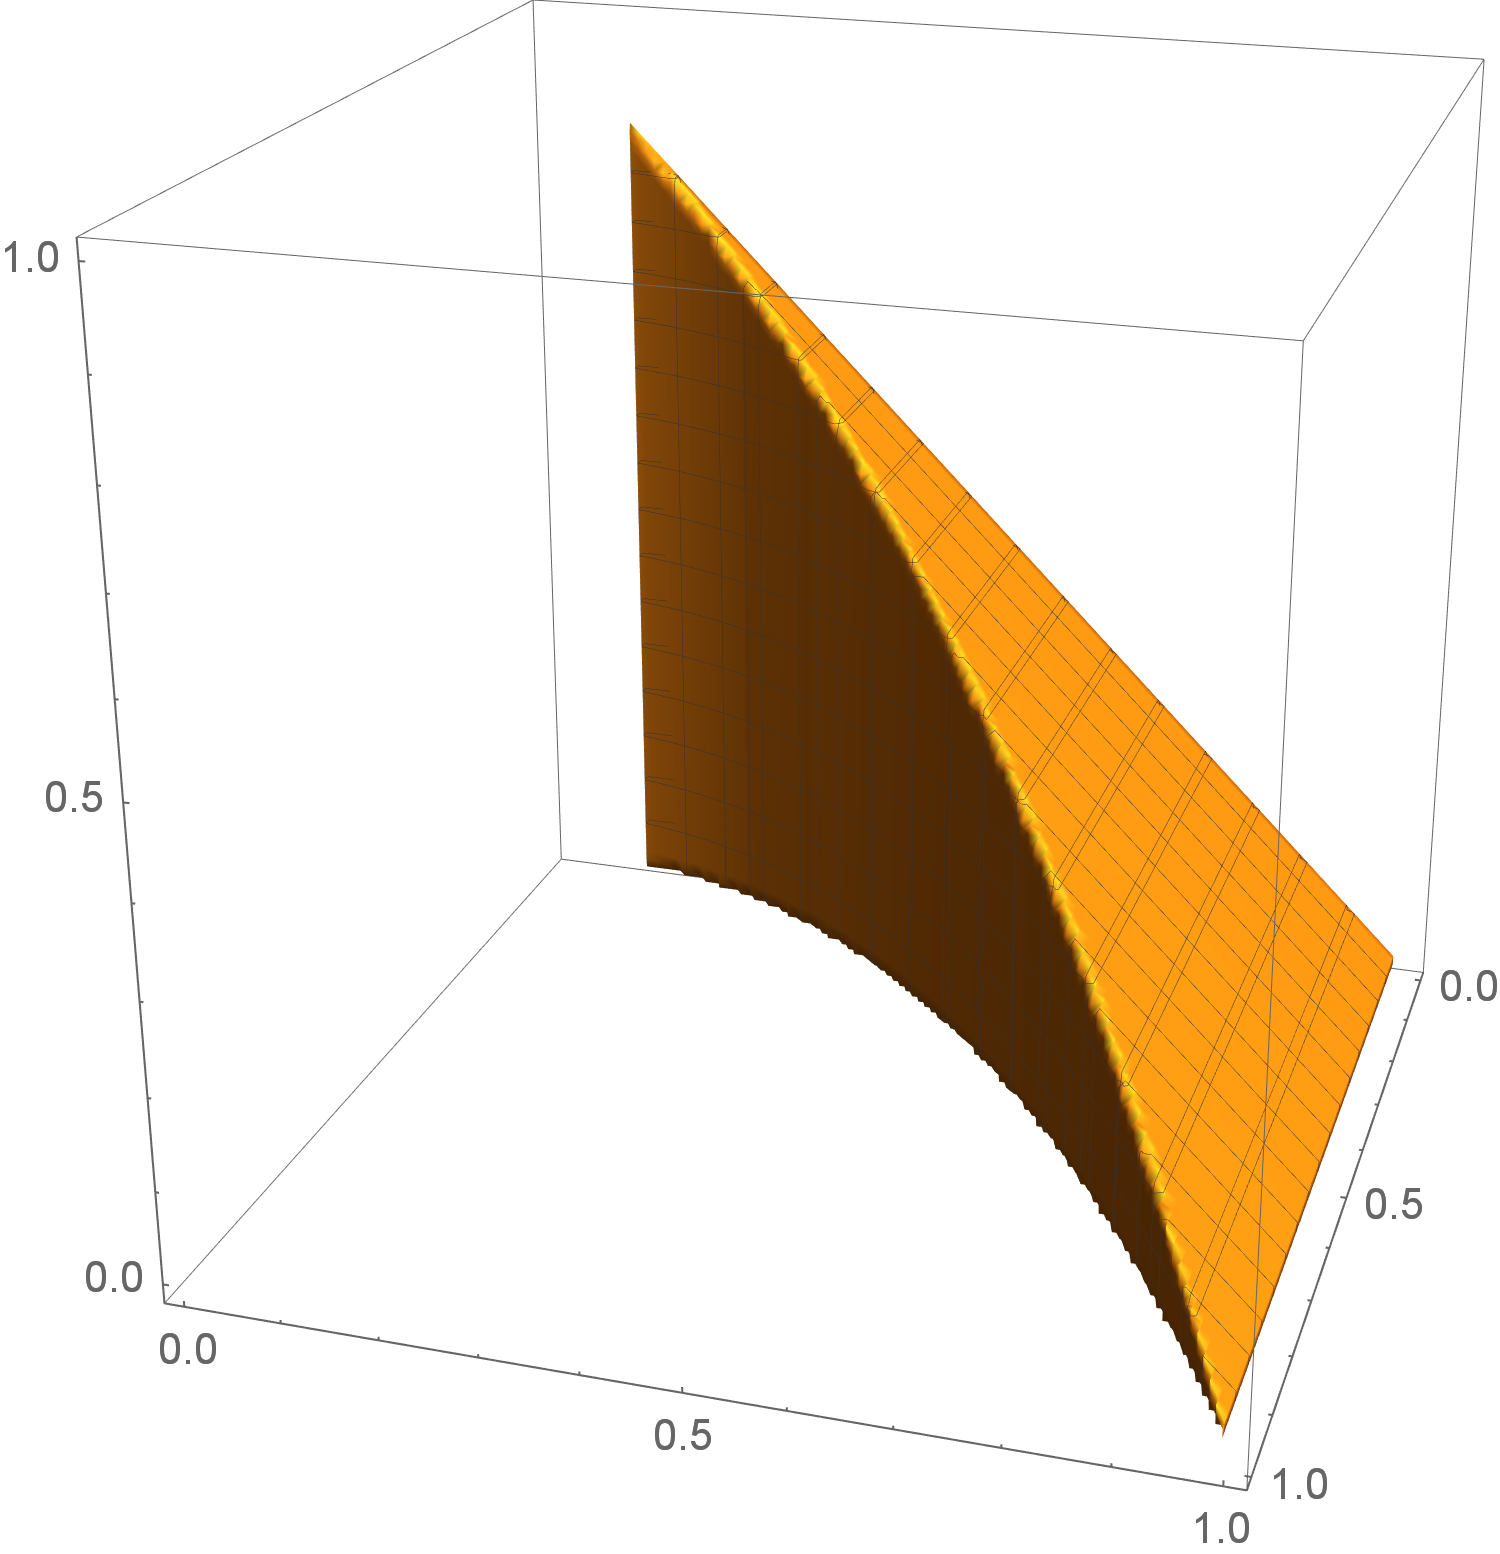
\includegraphics{threeRegion1.png}
  \end{image}
  Set up \textbf{six} iterated integrals that compute the volume of this solid,
  all which integrate in a different order.
\end{problem}


\end{document}
